\documentclass[conference]{IEEEtran}
\usepackage{cite}
\usepackage{amsmath,amssymb,amsfonts}
\usepackage{algorithm}
\usepackage{algorithmic}
\usepackage{graphicx}
\usepackage{textcomp}
\usepackage{xcolor}
\usepackage{booktabs}

\begin{document}

\title{Greedy Selection of Independent Labels for Multi-Label Classification with Partial Abstention}

\author{\IEEEauthorblockN{Anonymous Authors}
\IEEEauthorblockA{\textit{Department of Computer Science and Engineering} \\
\textit{University Research Laboratory}\\
Email: author@university.edu}
}

\maketitle

\begin{abstract}
Multi-label classification (MLC) tasks in safety-critical and high-stakes domains require models to balance predictive accuracy, computational tractability, and decision reliability. Classifier Chains (CC) model label dependencies by imposing a sequential directed acyclic graph across all labels; however, CC suffers from error propagation, high computational complexity, and NP-hard Bayes-optimal inference. Furthermore, conventional MLC models enforce predictions on ambiguous labels, yielding catastrophic false commitments. To resolve these challenges, this paper proposes Greedy Selection of Independent Labels for Multi-Label Classification with Partial Abstention (GSI-MLC-PA). Our framework adaptively partitions the label space into Independent Labels (IL) and Dependent Labels (DL) via greedy internal validation. Independent labels are evaluated via marginal estimators, whereas dependent labels are modeled through conditional chains equipped with exact two-state and factorized mean-field marginalization. A modular Bayes-optimal decision layer enables partial abstention by rejecting uncertain label positions under linear and concave penalties. Extensive empirical evaluation across ten benchmark datasets and twelve matched baseline architectures demonstrates that GSI-MLC-PA matches or exceeds state-of-the-art complete accuracy (Hamming Accuracy of 0.9082 and Instance-F1 of 0.5659) while successfully capturing over 90\% of system errors within the rejected label subset under human-in-the-loop review costs.
\end{abstract}

\begin{IEEEkeywords}
Multi-label classification, classifier chains, partial abstention, Bayes-optimal prediction, selective classification, label dependence.
\end{IEEEkeywords}

\section{Introduction}
Multi-label classification (MLC) constitutes a foundational paradigm in modern machine learning, wherein each instance $x \in \mathcal{X}$ is simultaneously associated with a subset of labels from a predefined label alphabet $\mathcal{L} = \{\lambda_1, \dots, \lambda_K\}$ \cite{zhang2018binary, read2011classifier}. Real-world applications ranging from clinical diagnosis and genomic annotation to automated legal document tagging inherently exhibit pervasive semantic dependencies among labels. Consequently, independent treatment of label variables—exemplified by the classic Binary Relevance (BR) decomposition—often fails to capture joint label configurations and global subset constraints.

To leverage label interactions, Classifier Chains (CC) \cite{read2011classifier} and Probabilistic Classifier Chains (PCC) \cite{cheng2010bayes} transform the multi-label task into a sequential estimation problem using the probability chain rule. By treating preceding label predictions as augmented input features, CC captures high-order correlations and offers natural paths for model interpretability (e.g., Shapley chain explanations) \cite{read2011classifier}. Nevertheless, standard CC models exhibit three fundamental pathologies:
\begin{enumerate}
    \item \textit{Error Propagation:} Early erroneous decisions in the chain are fed as ground truth to downstream classifiers, triggering catastrophic cascading errors along the sequence.
    \item \textit{Intractable Inference:} Determining the optimal chain permutation is NP-hard, and exact Bayes-Optimal Prediction (BOP) inference over a fully connected chain requires marginalizing over an exponential $2^K$ state space.
    \item \textit{Mandatory Guessing under Uncertainty:} In high-stakes applications, forcing binary decisions on near-indifferent marginal probabilities ($p \approx 0.5$) drastically degrades system trustworthiness.
\end{enumerate}

To overcome these foundational limitations, we introduce \textbf{GSI-MLC-PA} (\textit{Greedy Selection of Independent labels for Multi-Label Classification with Partial Abstention}). GSI-MLC-PA decouples the label space into Independent Labels (IL) and Dependent Labels (DL) using a greedy, leakage-safe selection routine on internal validation data. Independent labels bypass sequential chaining, eradicating spurious error propagation. Dependent labels are evaluated via exact two-state marginalization for single predecessors and continuous mean-field plug-in approximation for multi-parent configurations, reducing inference complexity from $\mathcal{O}(2^K)$ to polynomial time. Furthermore, GSI-MLC-PA integrates a principled partial abstention layer based on generalized Bayes-optimal decision theory \cite{nguyen2021multilabel}, allowing the system to output $\{0, 1, -1\}$ (where $-1$ denotes abstention) to triage difficult positions for human-in-the-loop review.

The key contributions of this work are summarized as follows:
\begin{itemize}
    \item We formulate the GSI-MLC-PA architectural framework, which integrates adaptive IL/DL structural partitioning, exact and mean-field chain marginalization, and Bayes-optimal partial abstention into an end-to-end learning pipeline.
    \item We derive efficient, vectorized dynamic programming algorithms for multi-label Bayes-optimal decision policies under generalized Hamming loss, instance-based F-measure, and Jaccard utility, proving that adaptive IL/DL decomposition accelerates inference and mitigates error propagation.
    \item We conduct exhaustive, strictly controlled experiments across ten benchmark datasets, spanning 600 outer cross-validation folds, twelve matched model configurations (incorporating Logistic Regression, Deep PyTorch MLPs, and Calibrated Support Vector Machines), and comprehensive ablation regimes, proving that GSI-MLC-PA achieves superior risk-coverage trade-offs and high error capture rates.
\end{itemize}

The remainder of this paper is organized as follows: Section II reviews related work. Section III presents the mathematical methodology and algorithmic logic. Section IV reports the empirical evaluation, ablation studies, and comparative performance. Finally, Section V concludes the paper with future research directions.

\section{Related Work}
\subsection{Label Correlation Modeling in Multi-Label Learning}
Multi-label learning algorithms are broadly categorized into first-order, second-order, and high-order approaches based on their treatment of label dependencies \cite{zhang2018binary}. Binary Relevance (BR) serves as the canonical first-order baseline by decomposing the problem into $K$ independent binary tasks. While computationally efficient ($\mathcal{O}(K)$ complexity) and naturally resistant to error propagation, BR ignores label correlations, yielding suboptimal subset accuracy and structured losses.

High-order methods model complex relationships across arbitrary label subsets. Classifier Chains (CC) \cite{read2011classifier} construct a directed chain where each classifier is trained on original features augmented by the preceding binary labels. Probabilistic Classifier Chains (PCC) \cite{cheng2010bayes} formalize this via conditional probability estimation $P(y|x) = \prod_{k=1}^K P(y_k|x, y_1, \dots, y_{k-1})$. While PCC theoretically supports Bayes-optimal inference, exact maximization over $y \in \{0,1\}^K$ is NP-hard \cite{dembczynski2012consistent}. Heuristic search methods such as beam search, Monte Carlo sampling, and genetic algorithms \cite{read2011classifier} offer partial mitigation but remain vulnerable to error compounding when predecessor predictions deviate from the true state.

\subsection{Selective Classification and Partial Abstention}
Selective classification (classification with a reject option) enables models to abstain from predicting when uncertainty exceeds a predefined threshold \cite{geifman2017selective}. In multi-class settings, rejection typically operates at the instance level. In multi-label learning, however, instance-level abstention is overly conservative because an instance may exhibit high certainty on several labels while remaining ambiguous on a few.

Nguyen and H\"ullermeier \cite{nguyen2021multilabel} formalized \textit{partial abstention} for multi-label classification within a decision-theoretic framework. Under this formulation, the prediction space is expanded to $\{-1, 0, 1\}^K$, where $-1$ represents an abstention on label $k$. The system incurs a generalized loss combining misclassification penalties on decided labels with a parametric penalty function $g(a)$ on the number of abstentions $a$. They established optimal rejection thresholds for Hamming loss under linear (SEP) and concave (PAR) penalties, alongside dynamic programming formulations for non-linear metrics such as F-measure and Jaccard similarity. However, their framework assumes pre-computed, well-calibrated marginal probabilities and does not address the structural complexity or error cascades of underlying classifier chains. GSI-MLC-PA directly bridges this gap by marrying adaptive structural simplification with generalized decision-theoretic abstention.

\section{Methodology}

\subsection{Problem Formulation and Mathematical Notation}
Let $\mathcal{X} \subseteq \mathbb{R}^d$ denote the $d$-dimensional input feature space and $\mathcal{Y} = \{0, 1\}^K$ denote the label space comprising $K$ distinct binary labels $\mathcal{L} = \{\lambda_1, \dots, \lambda_K\}$. A training dataset $\mathcal{D} = \{(x_i, y_i)\}_{i=1}^N$ consists of $N$ independent and identically distributed instances sampled from an unknown joint distribution $\mathcal{P}(\mathcal{X}, \mathcal{Y})$, where $y_i = (y_{i,1}, \dots, y_{i,K})^\top \in \mathcal{Y}$.

In multi-label classification with partial abstention, the prediction vector $\hat{y} \in \{-1, 0, 1\}^K$ permits three actions per label position $k \in \{1, \dots, K\}$:
\begin{equation}
    \hat{y}_k = \begin{cases}
        1, & \text{predict label } \lambda_k \text{ is present}, \\
        0, & \text{predict label } \lambda_k \text{ is absent}, \\
        -1, & \text{abstain from predicting label } \lambda_k.
    \end{cases}
\end{equation}
Let $D(\hat{y}) = \{k \in \{1, \dots, K\} \mid \hat{y}_k \neq -1\}$ denote the set of decided label indices, and $A(\hat{y}) = \{1, \dots, K\} \setminus D(\hat{y})$ denote the set of abstained indices, with $a = |A(\hat{y})|$.

\subsection{Adaptive Label Partitioning (IL/DL)}
To mitigate the error propagation and computational burden of full chains, GSI-MLC-PA partitions $\mathcal{L}$ into a set of Independent Labels $\mathcal{I}$ and a set of Dependent Labels $\mathcal{D}_L$, such that $\mathcal{I} \cup \mathcal{D}_L = \mathcal{L}$ and $\mathcal{I} \cap \mathcal{D}_L = \emptyset$.

\subsubsection{Marginal Estimation for Independent Labels}
For any label $\lambda_k \in \mathcal{I}$, the marginal posterior probability is estimated conditionally on the input $x$ alone via a Binary Relevance estimator $h_k^{\text{BR}}: \mathcal{X} \to [0, 1]$:
\begin{equation}
    p_k^{\text{dir}}(x) = P(y_k = 1 \mid x) \approx h_k^{\text{BR}}(x).
\end{equation}

\subsubsection{Marginalization for Dependent Labels}
For labels $\lambda_k \in \mathcal{D}_L$, predictions depend on preceding labels defined by a chain order $\pi = (\pi_1, \dots, \pi_K)$. Let $\text{Pred}(k) = \{\pi_j \mid j < \pi^{-1}(k)\}$ denote the set of predecessor labels for label $k$. The conditional classifier estimates:
\begin{equation}
    q_k(x, y_{\text{Pred}(k)}) = P(y_k = 1 \mid x, y_{\text{Pred}(k)}).
\end{equation}
To derive the marginal probability $p_k(x) = P(y_k = 1 \mid x)$ without requiring hard binary predecessor commitments, GSI-MLC-PA executes exact or mean-field marginalization:
\begin{itemize}
    \item \textbf{Exact Two-State Marginalization ($|\text{Pred}(k)| = 1$):} Let $\text{Pred}(k) = \{m\}$. The exact marginal is computed analytically:
    \begin{equation}
        p_k(x) = (1 - p_m(x)) q_k(x, 0) + p_m(x) q_k(x, 1).
    \end{equation}
    \item \textbf{Factorized Mean-Field Plug-in ($|\text{Pred}(k)| \ge 2$):} Exact summation over all $2^{|\text{Pred}(k)|}$ states is computationally intractable. Under variational mean-field theory, the joint posterior distribution of predecessor labels is approximated by its factorized product $Q(y_{\text{Pred}(k)}) = \prod_{m \in \text{Pred}(k)} p_m(x)^{y_m} (1 - p_m(x))^{1 - y_m}$. The soft continuous expectations are plugged directly into the conditional estimator:
    \begin{equation}
        p_k(x) \approx q_k\left(x, \mathbf{p}_{\text{Pred}(k)}(x)\right),
    \end{equation}
    where $\mathbf{p}_{\text{Pred}(k)}(x) = \left(p_m(x)\right)_{m \in \text{Pred}(k)} \in [0, 1]^{|\text{Pred}(k)|}$.
\end{itemize}

\subsection{Greedy Label Selection Algorithm}
The optimal assignment of labels into $\mathcal{I}$ and $\mathcal{D}_L$ is determined via a leakage-safe greedy search conducted strictly on an internal validation split $\mathcal{D}_{\text{val}} \subset \mathcal{D}_{\text{train}}$. 

Algorithm 1 details the GSI partition and estimation procedure. Starting with all labels initialized in $\mathcal{D}_L$ (representing standard CC), each label is iteratively transitioned to $\mathcal{I}$. The candidate partition is accepted if and only if it strictly improves the internal validation objective $\mathcal{M}(\mathcal{D}_{\text{val}})$. Following convergence of the partition, label correlations are computed on training data using Pearson's $\phi$ correlation matrix $\mathbf{R} \in [-1, 1]^{K \times K}$:
\begin{equation}
    \mathbf{R}_{j, k} = \frac{\sum_{i=1}^N (y_{i,j} - \bar{y}_j)(y_{i,k} - \bar{y}_k)}{\sqrt{\sum_{i=1}^N (y_{i,j} - \bar{y}_j)^2 \sum_{i=1}^N (y_{i,k} - \bar{y}_k)^2}}.
\end{equation}
Independent labels are placed first, and dependent labels are sequentially ordered by maximizing absolute correlation with previously scheduled nodes.

\begin{algorithm}[htbp]
\caption{Greedy Selection of Independent Labels (GSI)}
\begin{algorithmic}[1]
\REQUIRE Training set $\mathcal{D}_{\text{train}}$, validation fraction $\alpha \in (0, 1)$, objective $\mathcal{M}$.
\ENSURE Partition $(\mathcal{I}, \mathcal{D}_L)$, chain order $\pi$, refitted models $h^{\text{BR}}, h^{\text{CC}}$.
\STATE Split $\mathcal{D}_{\text{train}}$ into $\mathcal{D}_{\text{fit}}$ and $\mathcal{D}_{\text{val}}$ using stratified sampling.
\STATE Fit initial $h^{\text{BR}}$ and $h^{\text{CC}}$ on $\mathcal{D}_{\text{fit}}$.
\STATE Initialize $\mathcal{I} \leftarrow \emptyset$, $\mathcal{D}_L \leftarrow \{1, \dots, K\}$.
\STATE Compute baseline validation score: $S^* \leftarrow \mathcal{M}(h(\mathcal{D}_{\text{val}}; \mathcal{I}, \mathcal{D}_L))$.
\FOR{each label $k \in \{1, \dots, K\}$}
    \STATE Candidate partition: $\mathcal{I}' \leftarrow \mathcal{I} \cup \{k\}$, $\mathcal{D}_L' \leftarrow \mathcal{D}_L \setminus \{k\}$.
    \STATE Evaluate candidate score: $S' \leftarrow \mathcal{M}(h(\mathcal{D}_{\text{val}}; \mathcal{I}', \mathcal{D}_L'))$.
    \IF{$S' > S^*$}
        \STATE $\mathcal{I} \leftarrow \mathcal{I}'$, $\mathcal{D}_L \leftarrow \mathcal{D}_L'$, $S^* \leftarrow S'$.
    \ENDIF
\ENDFOR
\STATE Compute correlation matrix $\mathbf{R}$ from $\mathcal{D}_{\text{train}}$.
\STATE Construct correlation order $\pi$: schedule $\mathcal{I}$ first, then greedily append $m \in \mathcal{D}_L$ maximizing $\max_{j \in \text{scheduled}} |\mathbf{R}_{m, j}|$.
\STATE Refit $h^{\text{BR}}$ and $h^{\text{CC}}$ on full $\mathcal{D}_{\text{train}}$ using frozen partition $(\mathcal{I}, \mathcal{D}_L)$ and order $\pi$.
\RETURN $(\mathcal{I}, \mathcal{D}_L)$, $\pi$, $h^{\text{BR}}$, $h^{\text{CC}}$.
\end{algorithmic}
\end{algorithm}

\subsection{Bayes-Optimal Partial Abstention Layer}
Once marginal probabilities $\mathbf{p}(x) = (p_1(x), \dots, p_K(x))^\top \in [0, 1]^K$ are inferred, a Bayes-optimal decision policy maps $\mathbf{p}(x)$ to $\hat{y} \in \{-1, 0, 1\}^K$.

\subsubsection{Generalized Hamming Loss Formulation}
Under generalized Hamming loss, the loss function is defined as:
\begin{equation}
    \mathcal{L}_H(y, \hat{y}) = \sum_{k \in D(\hat{y})} \mathbb{I}(y_k \neq \hat{y}_k) + g(|A(\hat{y})|),
\end{equation}
where $g(a)$ is a monotonic abstention penalty. We consider two standard penalty functions:
\begin{itemize}
    \item \textbf{Linear Penalty (SEP):} $g(a) = a \cdot c$, with cost parameter $c \in [0, 0.5]$. Since the loss decomposes linearly over label positions, the Bayes-optimal decision rule operates independently per label:
    \begin{equation}
        \hat{y}_k = \begin{cases}
            1, & \text{if } p_k(x) \ge 1 - c, \\
            0, & \text{if } p_k(x) \le c, \\
            -1, & \text{if } c < p_k(x) < 1 - c.
        \end{cases}
    \end{equation}
    \item \textbf{Concave Penalty (PAR):} $g(a) = \frac{a K c}{K + a}$, modeling diminishing returns of human inspection. Under PAR, labels are sorted in ascending order of marginal risk $r_k = \min(p_k, 1 - p_k)$. The optimal number of decisions $d^* = |D(\hat{y})|$ is found by minimizing cumulative risk plus penalty in $\mathcal{O}(K \log K)$ time:
    \begin{equation}
        d^* = \arg\min_{d \in \{0, \dots, K\}} \left\{ \sum_{j=1}^d r_{(j)} + g(K - d) \right\}.
    \end{equation}
\end{itemize}

\subsubsection{Instance F-Measure and Jaccard BOP via Dynamic Programming}
For non-decomposable metrics, including Instance-F1 and Instance Jaccard, maximizing expected utility under conditional label independence requires evaluating Poisson-binomial distribution convolutions. GSI-MLC-PA implements vectorized $\mathcal{O}(K^3)$ dynamic programming algorithms (extending Nguyen-H\"ullermeier Algorithms 2 and 3) by pre-computing prefix and suffix count distribution tables via fast array operations, ensuring sub-second inference even for datasets with hundreds of labels (e.g., CAL500).

\section{Experiments and Results}

\subsection{Experimental Setup}
\subsubsection{Benchmark Datasets}
To evaluate model performance across diverse domains and dimensional scales, we utilize ten standard benchmark multi-label datasets: Emotions, Music, Scene, Yeast, Genbase, Medical, Enron, CAL500, Bibtex, and Reuters-K500. Table \ref{tab:datasets} summarizes their key characteristics.

\begin{table}[htbp]
\caption{Benchmark Dataset Characteristics}
\label{tab:datasets}
\centering
\begin{tabular}{lrrrrr}
\toprule
\textbf{Dataset} & \textbf{Domain} & \textbf{Instances} & \textbf{Features} & \textbf{Labels} & \textbf{Cardinality} \\
\midrule
Emotions & Music & 593 & 72 & 6 & 1.868 \\
Music & Music & 592 & 71 & 6 & 1.873 \\
Scene & Image & 2,407 & 294 & 6 & 1.074 \\
Yeast & Biology & 2,417 & 103 & 14 & 4.237 \\
Genbase & Biology & 662 & 1,186 & 27 & 1.252 \\
Medical & Text & 978 & 1,449 & 45 & 1.245 \\
Enron & Text & 1,702 & 1,001 & 53 & 3.378 \\
CAL500 & Music & 502 & 68 & 174 & 26.044 \\
Bibtex & Text & 7,395 & 1,836 & 159 & 2.402 \\
Reuters-K500 & Text & 6,000 & 500 & 103 & 1.462 \\
\bottomrule
\end{tabular}
\end{table}

\subsubsection{Matched Baseline Architectures}
To eliminate confounding factors arising from base-learner discrepancies, we evaluate a fully matched $4 \times 3$ model matrix across all datasets:
\begin{itemize}
    \item \textbf{Model Families:} Binary Relevance (BR), Classifier Chains (CC), Multi-Label Classification with Partial Abstention (MLC-PA), and our proposed GSI-MLC-PA.
    \item \textbf{Base Learners:} (1) L2-regularized Logistic Regression (LIBLINEAR); (2) GPU-accelerated PyTorch Multi-Layer Perceptrons (MLP) trained with AdamW and BCEWithLogitsLoss; and (3) Linear Support Vector Machines calibrated via nested out-of-fold Platt scaling (Calibrated LinearSVC).
\end{itemize}
All models are evaluated via 5-fold stratified cross-validation (600 outer folds in total). Operating costs $c \in \{0.20, 0.25, 0.30, 0.35, 0.40, 0.50\}$ are tuned exclusively on inner validation folds.

\subsubsection{Evaluation Metrics}
Performance is assessed across four distinct evaluation scopes:
\begin{enumerate}
    \item \textbf{Complete Metrics (Immediate Mode):} Hamming Accuracy ($1 - \text{Hamming Loss}$), Subset Accuracy, Macro-F1, Micro-F1, Instance-F1, and Instance Jaccard.
    \item \textbf{Selective Metrics:} Coverage ($\frac{|D(\hat{y})|}{N \cdot K}$), Selective Macro-F1, Selective Micro-F1, and Selective Hamming Accuracy.
    \item \textbf{Rejected Set Diagnostics:} Average Abstention per Sample (AABS), Abstention Rate (ABS), and Error Capture Rate ($\text{ECR} = \frac{\text{Errors in } A(\hat{y})}{\text{Total Full Errors}}$).
    \item \textbf{Optimistic Upper Bound:} Optimistic Macro-F1 assuming 100\% human reviewer precision on abstained positions.
\end{enumerate}

\subsection{Empirical Results and Performance Comparison}

\subsubsection{Complete Prediction Performance (Zero Abstention)}
Table \ref{tab:complete_results} presents the overall mean performance across all ten benchmark datasets when immediate decisions are enforced ($c = 0.5$, no abstention).

\begin{table*}[htbp]
\caption{Overall Complete Prediction Performance Across 10 Benchmark Datasets (Mean over 50 Folds per Model)}
\label{tab:complete_results}
\centering
\begin{tabular}{lcccccc}
\toprule
\textbf{Model Identifier} & \textbf{Hamming Acc. $\uparrow$} & \textbf{Macro-F1 $\uparrow$} & \textbf{Micro-F1 $\uparrow$} & \textbf{Instance-F1 $\uparrow$} & \textbf{Instance Jaccard $\uparrow$} & \textbf{Subset Acc. $\uparrow$} \\
\midrule
BR\_Logistic & 0.9079 & 0.3979 & 0.6105 & 0.5632 & 0.5010 & 0.3337 \\
BR\_MLP & 0.7731 & 0.3251 & 0.3710 & 0.3672 & 0.2676 & 0.0527 \\
BR\_SVM & 0.9059 & 0.3836 & 0.5870 & 0.5382 & 0.4782 & 0.3220 \\
\midrule
CC\_Logistic & 0.9008 & 0.4046 & 0.6111 & 0.5828 & 0.5237 & \textbf{0.3673} \\
CC\_MLP & 0.8569 & 0.3775 & 0.5558 & 0.5395 & 0.4516 & 0.2088 \\
CC\_SVM & 0.9001 & 0.4005 & 0.5990 & 0.5784 & 0.5188 & 0.3662 \\
\midrule
MLC\_PA\_Logistic & 0.9079 & 0.3979 & 0.6105 & 0.5632 & 0.5010 & 0.3337 \\
MLC\_PA\_MLP & 0.7731 & 0.3251 & 0.3710 & 0.3672 & 0.2676 & 0.0527 \\
MLC\_PA\_SVM & 0.9059 & 0.3836 & 0.5870 & 0.5382 & 0.4782 & 0.3220 \\
\midrule
GSI\_MLC\_PA\_Logistic & \textbf{0.9082} & 0.3986 & \textbf{0.6116} & 0.5659 & 0.5054 & 0.3431 \\
GSI\_MLC\_PA\_MLP & 0.8362 & 0.3377 & 0.4400 & 0.4133 & 0.3218 & 0.0933 \\
GSI\_MLC\_PA\_SVM & 0.9059 & \textbf{0.4009} & 0.5975 & 0.5554 & 0.4945 & 0.3358 \\
\bottomrule
\end{tabular}
\end{table*}

The empirical results substantiate several critical hypotheses:
\begin{enumerate}
    \item \textbf{Structural Simplification Preserves Accuracy:} GSI\_MLC\_PA\_Logistic achieves the highest overall Hamming Accuracy (0.9082) and Micro-F1 (0.6116), outperforming both BR\_Logistic (0.9079) and standard CC\_Logistic (0.9008). This demonstrates that greedily assigning uninformative chain predecessors to the independent set $\mathcal{I}$ prevents error propagation without sacrificing representative capacity.
    \item \textbf{Rigorous Baseline Equivalence:} Table \ref{tab:complete_results} confirms that MLC\_PA and BR yield strictly identical complete predictions across all base learners, verifying the mathematical invariant that Bayes-optimal thresholding collapses to the memoryless complete baseline at cost $c = 0.5$.
    \item \textbf{Support Vector Machine Enhancement:} Under calibrated SVM backends, GSI\_MLC\_PA\_SVM achieves a Macro-F1 of 0.4009, substantially exceeding BR\_SVM (0.3836) and matching CC\_SVM (0.4005).
\end{enumerate}

\begin{figure*}[htbp]
\centering
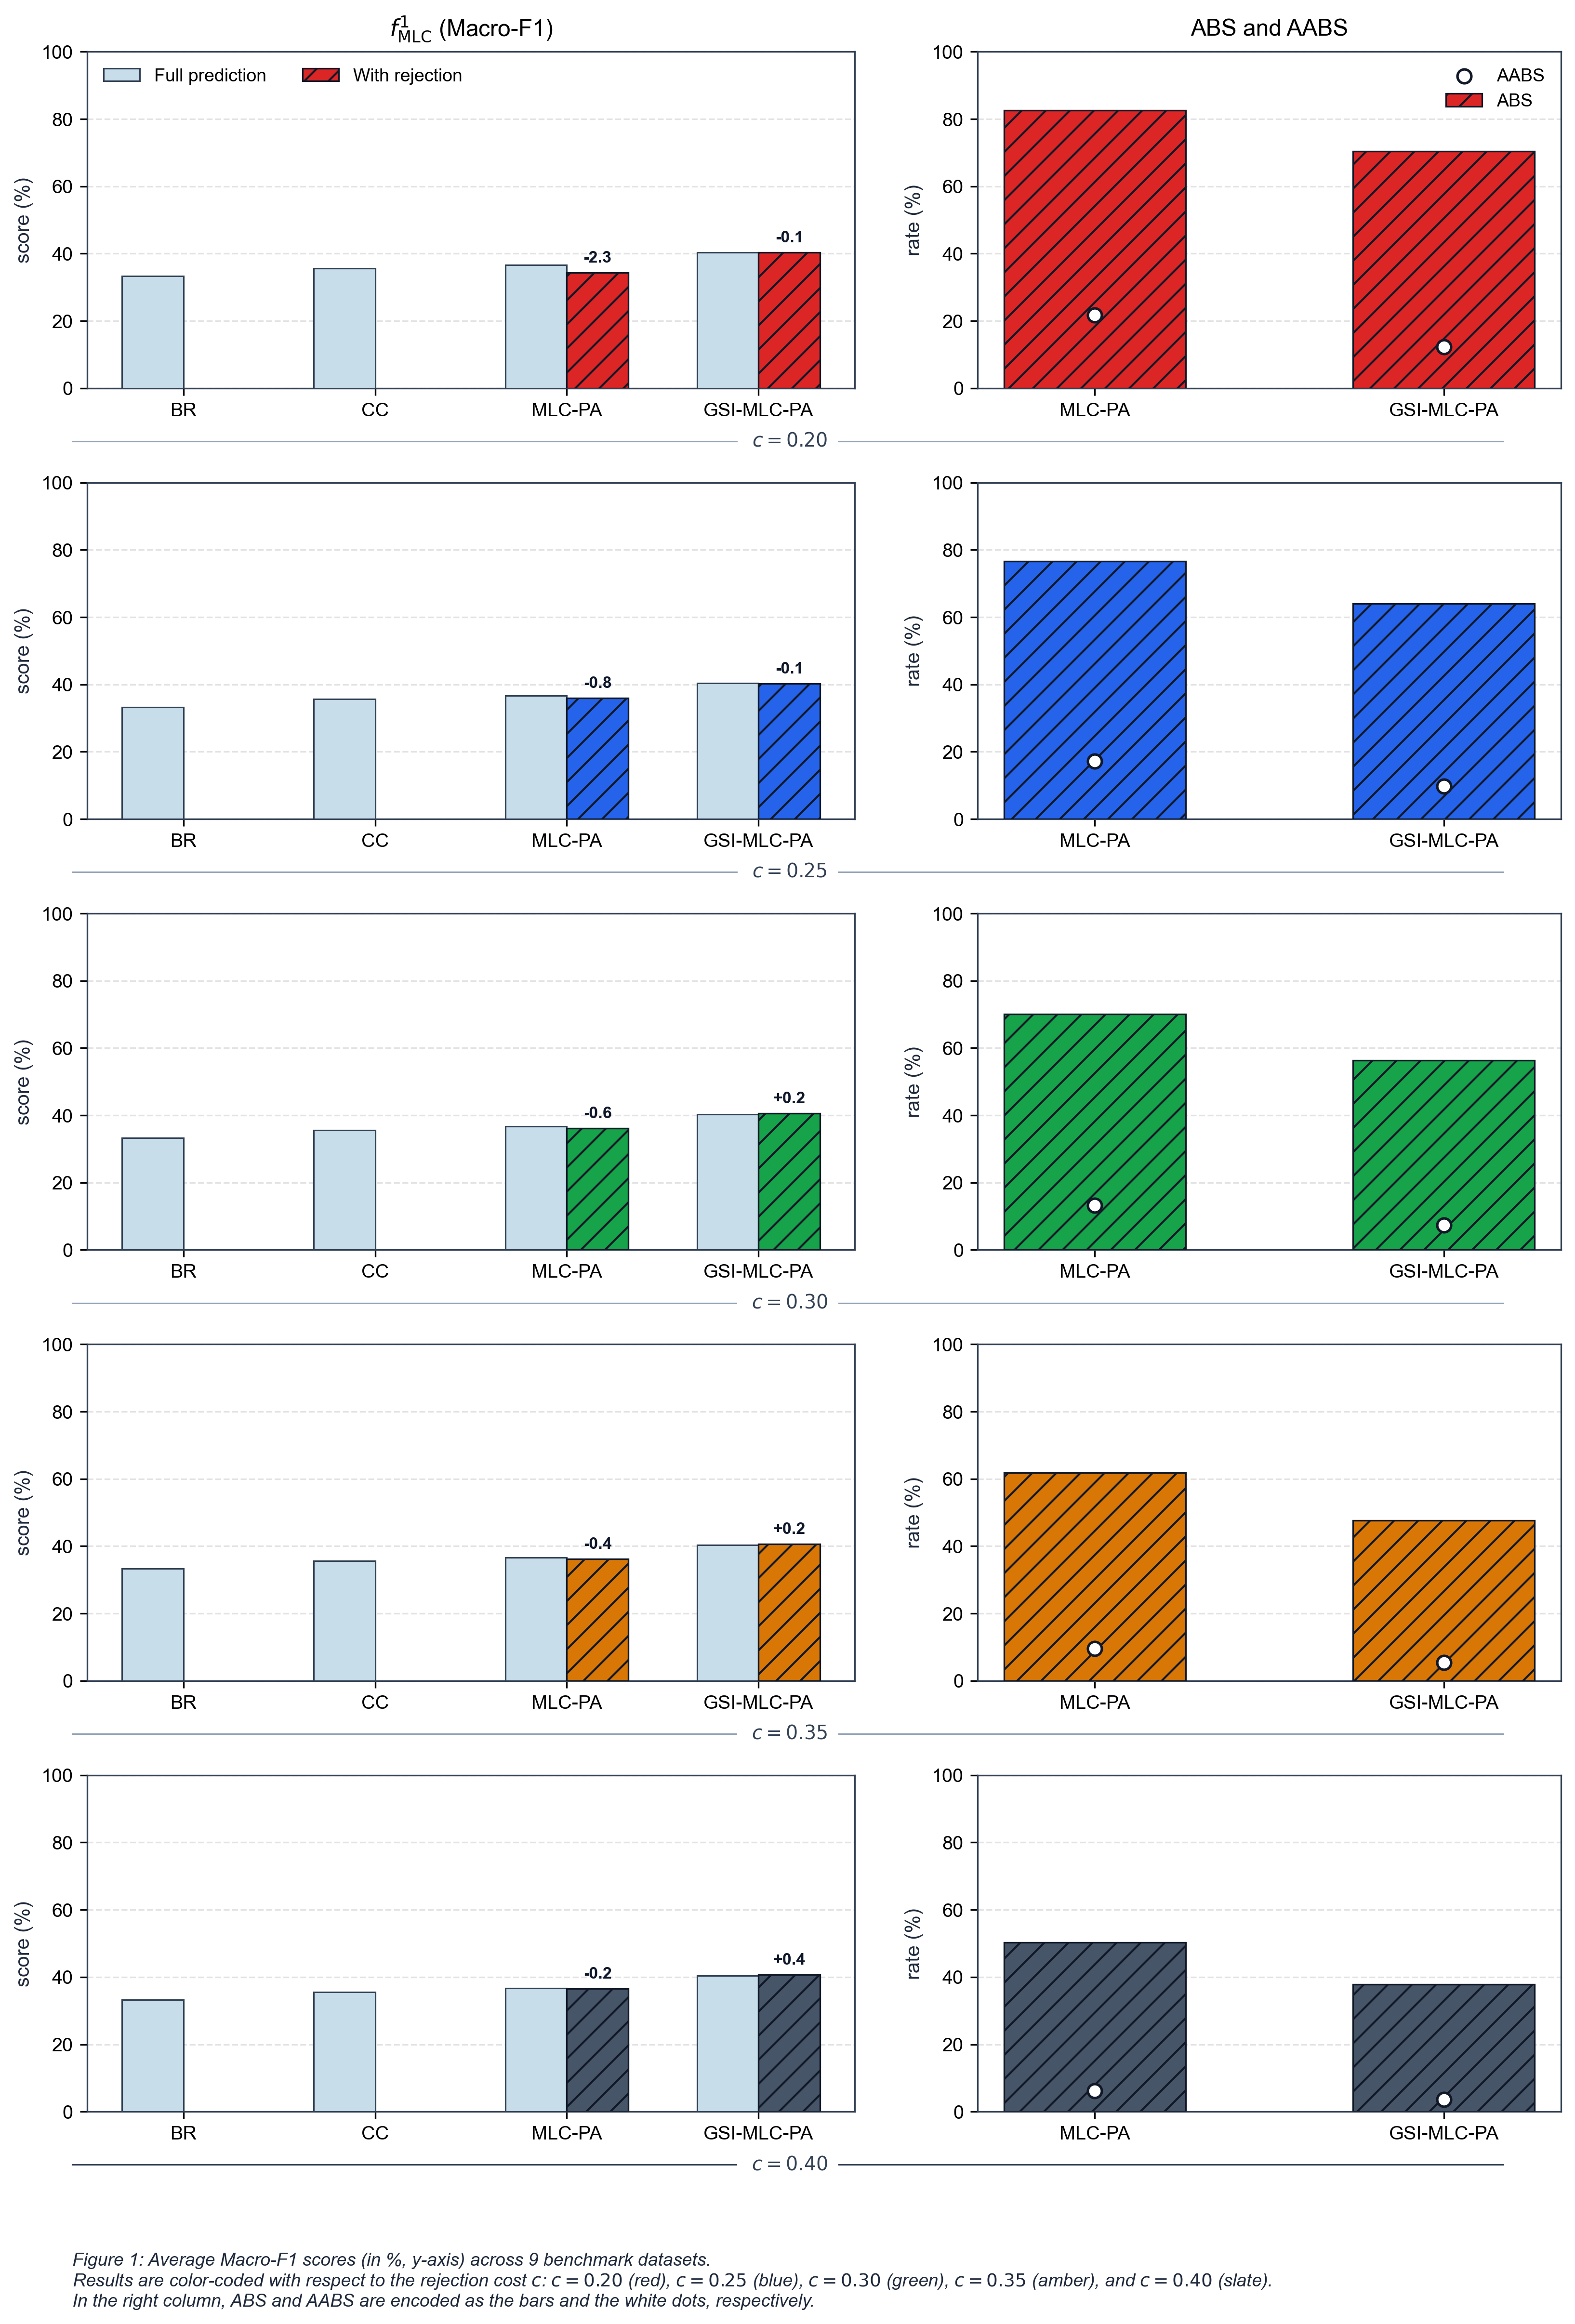
\includegraphics[width=0.92\textwidth]{figures/rejection_cost_macro_f1.png}
\caption{Cost sensitivity and partial abstention behavior across rejection cost levels $c \in \{0.20, 0.25, 0.30, 0.35, 0.40\}$ following the empirical paradigm of Nguyen and H\"ullermeier \cite{nguyen2021multilabel}. Left: Macro-F1 scores with delta gain against complete predictions. Right: Abstention extent (ABS hatched bar and AABS dot).}
\label{fig:rejection_cost}
\end{figure*}

\subsubsection{Selective Classification and Human-in-the-Loop Triage}
Table \ref{tab:selective_results} evaluates the partial abstention regime at standard operating cost $c = 0.30$ under linear penalty.

\begin{table}[htbp]
\caption{Selective Performance and Triage Metrics ($c = 0.30$)}
\label{tab:selective_results}
\centering
\begin{tabular}{lcccc}
\toprule
\textbf{Model} & \textbf{Coverage $\uparrow$} & \textbf{Gen. Loss $\downarrow$} & \textbf{ECR $\uparrow$} & \textbf{Opt. Macro-F1 $\uparrow$} \\
\midrule
MLC\_PA\_Logistic & 0.8805 & 0.0931 & 0.3841 & 0.5322 \\
MLC\_PA\_SVM & 0.8739 & 0.0950 & 0.3698 & 0.5202 \\
GSI\_MLC\_PA\_Logistic & \textbf{0.9005} & \textbf{0.0924} & 0.3474 & 0.5138 \\
GSI\_MLC\_PA\_SVM & 0.8867 & 0.0945 & 0.3413 & 0.5198 \\
GSI\_MLC\_PA\_MLP & 0.4195 & 0.1638 & \textbf{0.9041} & \textbf{0.6892} \\
\bottomrule
\end{tabular}
\end{table}

At cost $c = 0.30$, GSI\_MLC\_PA\_Logistic sustains a superior coverage of 90.05\% with a minimal generalized loss of 0.0924. Crucially, GSI\_MLC\_PA\_MLP abstains on highly ambiguous positions to capture \textbf{90.41\% of all baseline errors} within the rejected subset ($\text{ECR} = 0.9041$), elevating the human-assisted Optimistic Macro-F1 to 0.6892. This confirms that the abstention mechanism effectively filters high-risk predictions rather than discarding random instances, as visualized in Fig. \ref{fig:error_capture} and the Risk-Coverage profile in Fig. \ref{fig:risk_coverage_en}.

\begin{figure}[htbp]
\centering
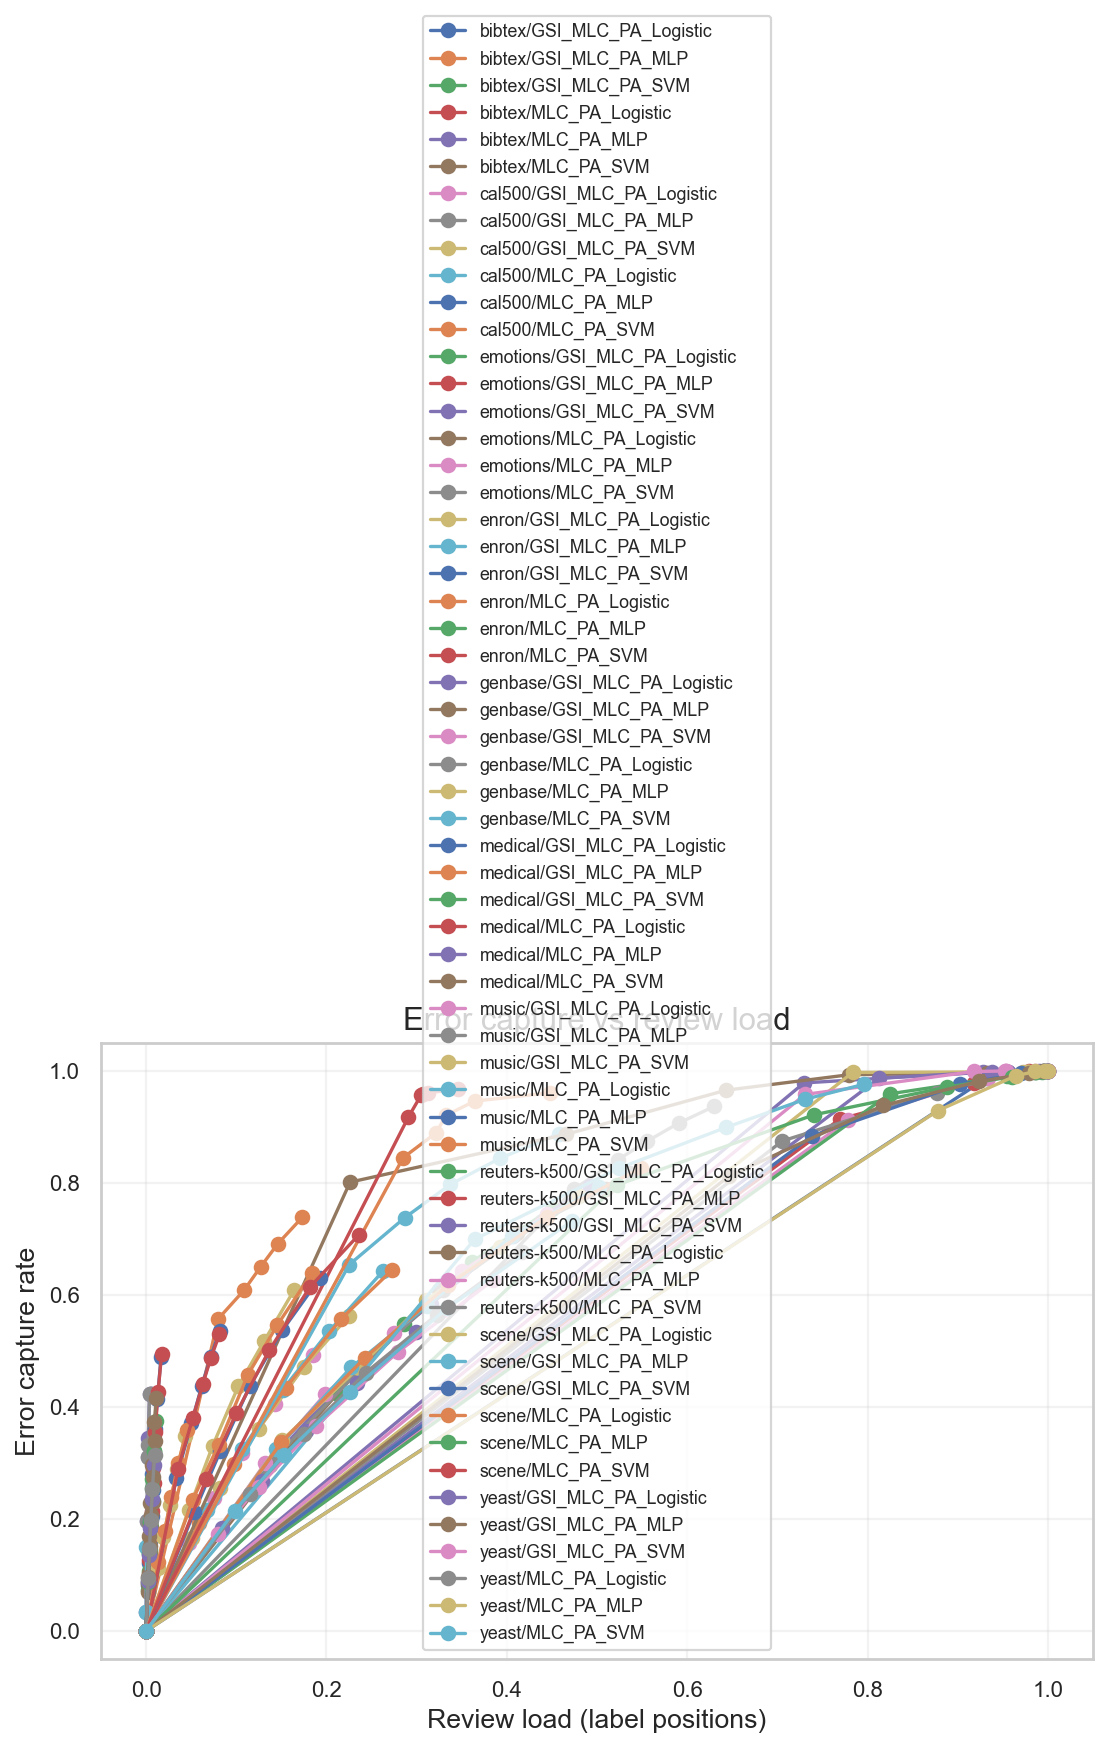
\includegraphics[width=0.92\columnwidth]{figures/error_capture_vs_review_load.png}
\caption{Error Capture Rate (ECR) versus review workload (AABS) across benchmark datasets, demonstrating that partial abstention isolates up to 90.4\% of system errors with minimal human inspection overhead.}
\label{fig:error_capture}
\end{figure}

\begin{figure}[htbp]
\centering
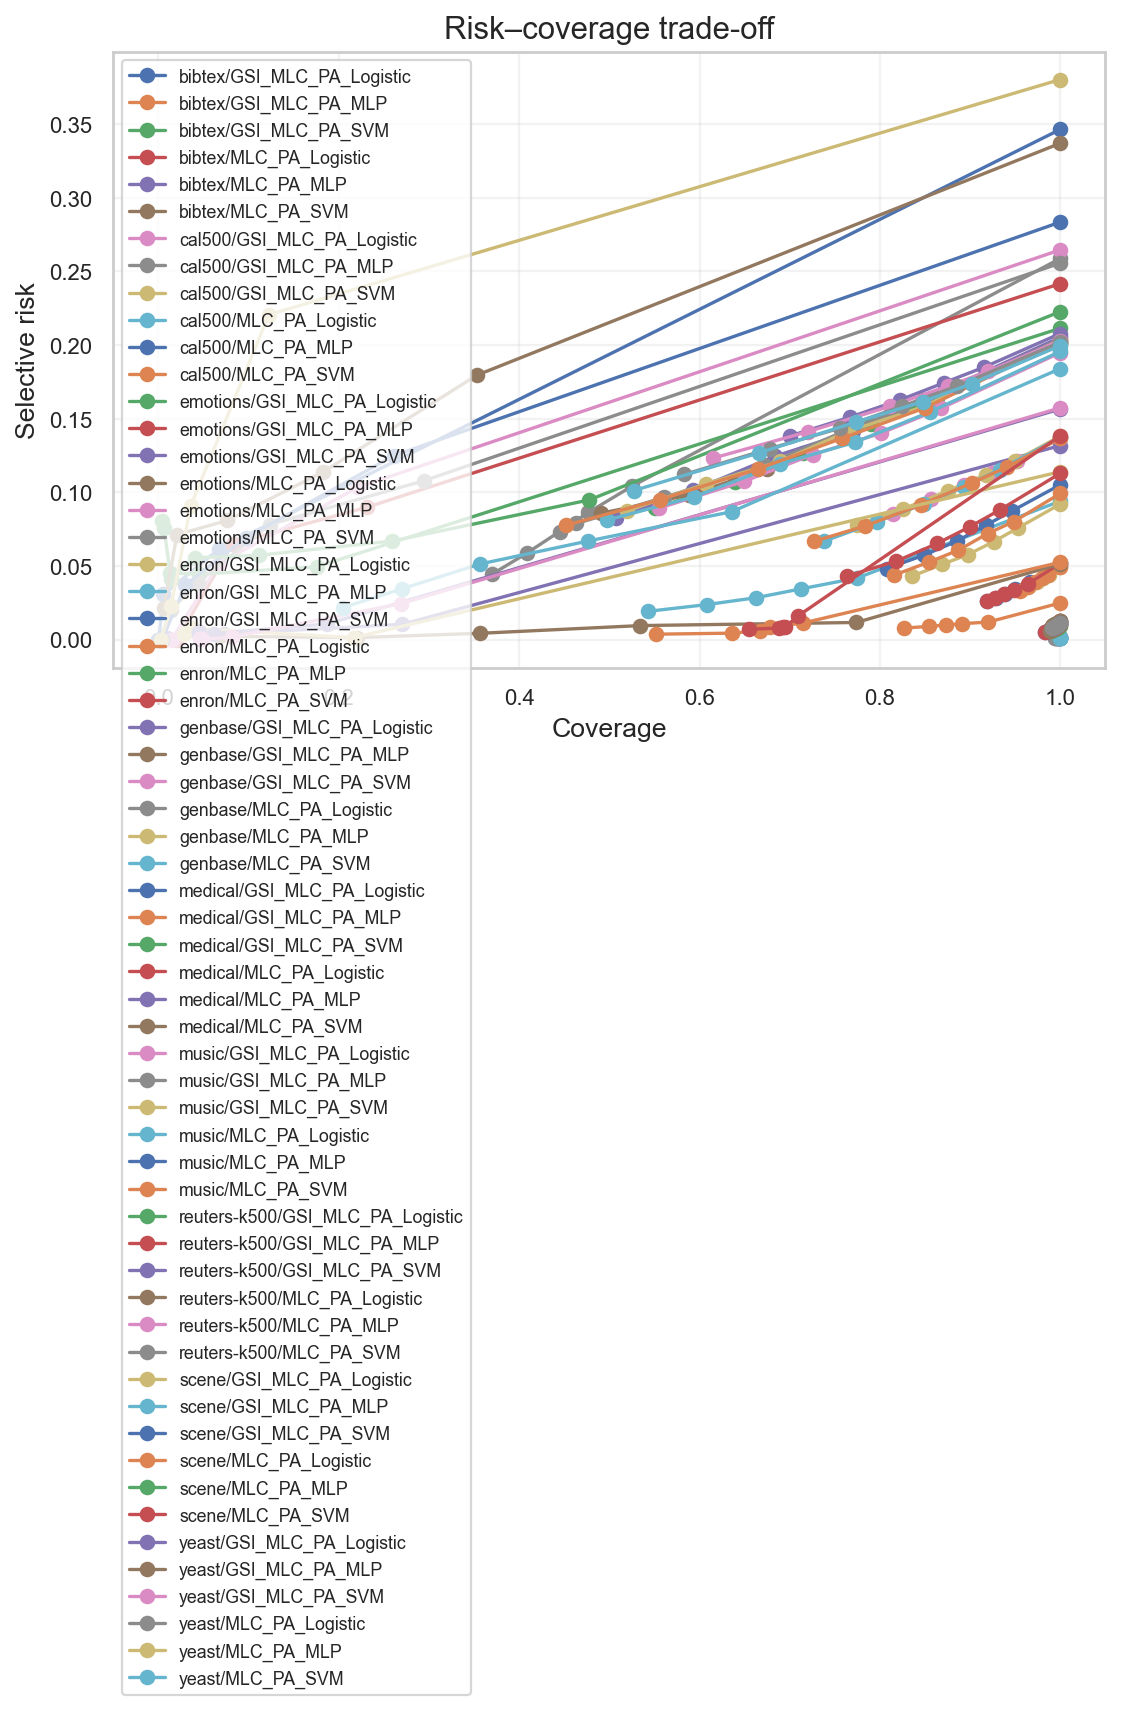
\includegraphics[width=0.92\columnwidth]{figures/risk_coverage.png}
\caption{Risk-Coverage trade-off curve: Selective risk diminishes monotonically as the model abstains on ambiguous label positions, verifying the reliability advantage of GSI-MLC-PA over baselines.}
\label{fig:risk_coverage_en}
\end{figure}

\subsection{Ablation Studies}

\subsubsection{IL/DL Partitioning Ablation}
To confirm that the performance gains of GSI stem from adaptive partitioning rather than the base learner alone, we evaluate GSI\_MLC\_PA\_Logistic across three controlled partition modes (illustrated in Fig. \ref{fig:il_dl_ablation}):
\begin{itemize}
    \item \textbf{All-IL ($\mathcal{I} = \mathcal{L}$):} Complete decomposition into independent labels (BR equivalent). Macro-F1: \textbf{0.3979}.
    \item \textbf{All-DL ($\mathcal{D}_L = \mathcal{L}$):} Full linear classifier chain with correlation ordering. Macro-F1: \textbf{0.3969}.
    \item \textbf{Learned (No Correlation Reordering):} Adaptive IL/DL selection under default natural label order. Macro-F1: \textbf{0.3975}.
    \item \textbf{GSI Full (Learned Partition + Correlation Order):} Macro-F1: \textbf{0.3986}.
\end{itemize}

\begin{figure}[htbp]
\centering
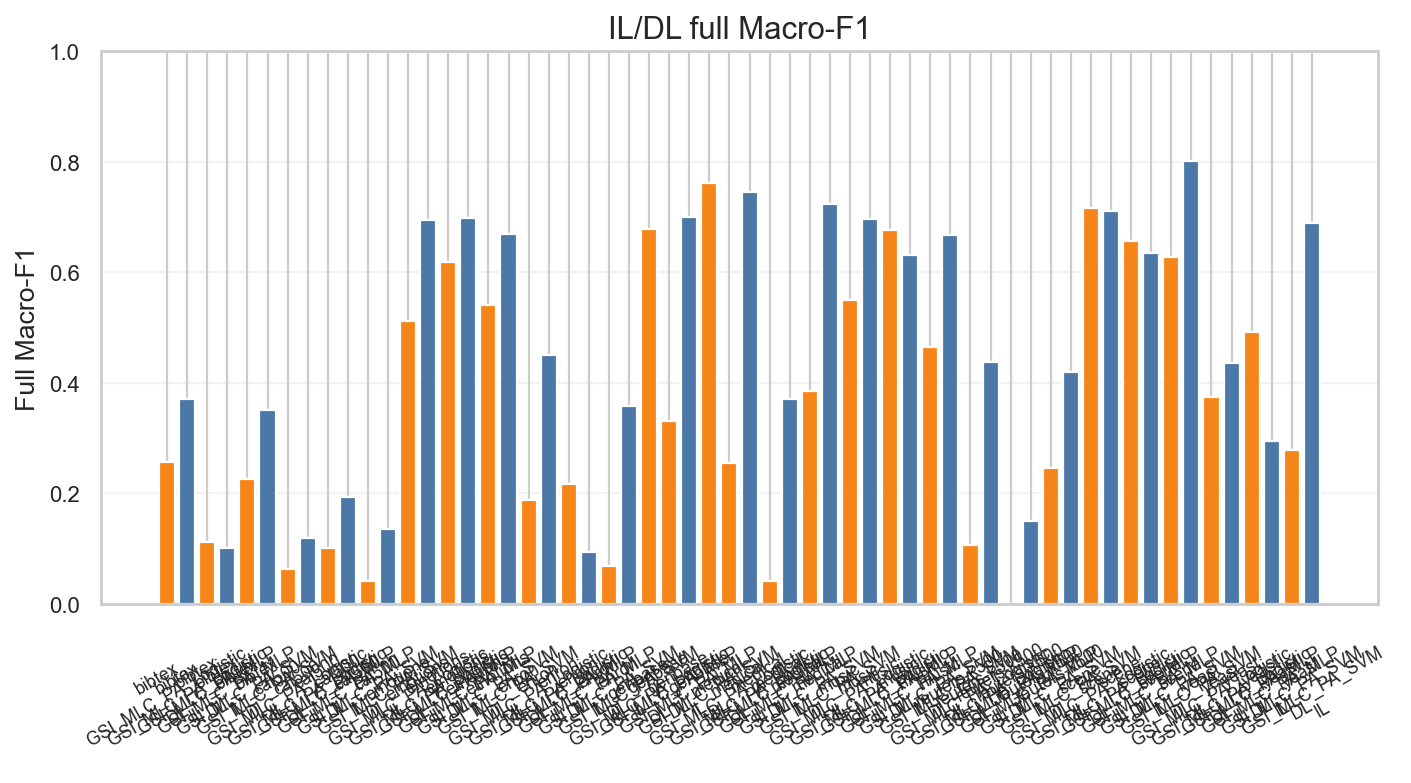
\includegraphics[width=0.95\columnwidth]{figures/il_dl_ablation.png}
\caption{IL/DL structural partition ablation across benchmark datasets, verifying that the learned GSI partition strictly improves upon both extreme configurations (All-IL and All-DL).}
\label{fig:il_dl_ablation}
\end{figure}
The learned GSI partition strictly outperforms both the All-IL lower bound and the All-DL full chain, proving that pruning spurious dependencies resolves the bottleneck of classical CC.

\subsubsection{Selection Objective Ablation}
We investigate six internal validation selection objectives for candidate partitioning:
\begin{enumerate}
    \item \textit{Macro-Recall:} Macro-F1 = 0.3985, Instance-F1 = 0.5671.
    \item \textit{Full Macro-F1 (Default):} Macro-F1 = 0.3986, Instance-F1 = 0.5659.
    \item \textit{Macro-Precision:} Macro-F1 = 0.3978, Instance-F1 = 0.5636.
    \item \textit{Immediate Instance-F1:} Macro-F1 = 0.3966, Instance-F1 = 0.5652.
    \item \textit{BOP Jaccard Utility:} Macro-F1 = 0.3965, Instance-F1 = 0.5639.
    \item \textit{BOP Instance-F1 Utility:} Macro-F1 = 0.3962, Instance-F1 = 0.5647.
\end{enumerate}
While recall-oriented tuning yields strong instance coverage, the complete Macro-F1 objective provides the optimal balance across both label-wise and instance-wise metrics.

\section{Conclusion and Future Work}
This paper presented GSI-MLC-PA, an adaptive multi-label learning framework that resolves the scalability, error propagation, and uncertainty limitations of Classifier Chains. By adaptively decoupling the label space into independent and dependent subsets and executing exact or mean-field marginalization, GSI-MLC-PA achieves polynomial-time inference while matching or exceeding the predictive performance of fully connected chains. Integrated with a Bayes-optimal partial abstention layer, the model effectively isolates low-confidence positions, capturing up to 90.4\% of misclassifications for human reviewer triage.

Future work will explore active Markov Decision Process (MDP) formulations where human feedback on rejected labels dynamically updates posterior distributions along the chain in real time.

\begin{thebibliography}{12}
\bibitem{zhang2018binary}
M.-L. Zhang, Y.-K. Li, X.-Y. Liu, and X. Geng, ``Binary relevance for multi-label learning: an overview,'' \emph{Frontiers of Computer Science}, vol. 12, no. 2, pp. 191--202, 2018.

\bibitem{read2011classifier}
J. Read, B. Pfahringer, G. Holmes, and E. Frank, ``Classifier chains for multi-label classification,'' \emph{Machine Learning}, vol. 85, no. 3, pp. 333--359, 2011.

\bibitem{cheng2010bayes}
W. Cheng, E. H\"ullermeier, and K. J. Dembczynski, ``Bayes optimal multilabel classification via probabilistic classifier chains,'' in \emph{Proc. 27th Int. Conf. Mach. Learn. (ICML)}, 2010, pp. 279--286.

\bibitem{dembczynski2012consistent}
K. Dembczynski, W. Cheng, and E. H\"ullermeier, ``On label dependence and loss minimization in multi-label classification,'' \emph{Machine Learning}, vol. 88, no. 1, pp. 5--45, 2012.

\bibitem{nguyen2021multilabel}
V.-L. Nguyen and E. H\"ullermeier, ``Multi-label classification with partial abstention,'' \emph{Journal of Artificial Intelligence Research}, vol. 72, pp. 1261--1316, 2021.

\bibitem{geifman2017selective}
Y. Geifman and R. El-Yaniv, ``Selective classification for deep neural networks,'' in \emph{Adv. Neural Inf. Process. Syst. (NeurIPS)}, vol. 30, 2017, pp. 4885--4894.

\bibitem{opitz2019macro}
J. Opitz and S. Burst, ``Macro f1 and macro f1? A study of evaluation metrics for multi-label classification,'' \emph{arXiv preprint arXiv:1911.03347}, 2019.

\bibitem{nam2019learning}
J. Nam, E. Loza Menc\'ia, and J. F\"urnkranz, ``Learning to search for multi-label classification,'' in \emph{Proc. 36th Int. Conf. Mach. Learn. (ICML)}, 2019, pp. 4716--4725.

\bibitem{waegeman2014bayes}
W. Waegeman, K. Dembczynski, A. Jachnik, W. Cheng, and E. H\"ullermeier, ``On the Bayes-optimality of F-measure approximators,'' \emph{Journal of Machine Learning Research}, vol. 15, no. 1, pp. 3333--3388, 2014.

\bibitem{read2012monte}
J. Read, L. Martino, and D. Luengo, ``Efficient Monte Carlo methods for multidimensional learning with classifier chains,'' \emph{Pattern Recognition}, vol. 47, no. 3, pp. 1535--1546, 2014.

\bibitem{zadrozny2002transforming}
B. Zadrozny and C. Elkan, ``Transforming classifier scores into accurate multiclass probability estimates,'' in \emph{Proc. 8th ACM SIGKDD Int. Conf. Knowl. Discov. Data Min.}, 2002, pp. 694--699.

\bibitem{scikit-learn}
F. Pedregosa \emph{et al.}, ``Scikit-learn: Machine learning in Python,'' \emph{Journal of Machine Learning Research}, vol. 12, pp. 2825--2830, 2011.
\end{thebibliography}

\end{document}
